\documentclass[10pt]{article}

%% Various useful packages and commands from different sources

\usepackage[applemac]{inputenc}
\usepackage[english]{babel}
\usepackage[T1]{fontenc}
\usepackage{cite, url,color} % Citation numbers being automatically sorted and properly "compressed/ranged".
%\usepackage{pgfplots}
\usepackage{graphics,amsfonts}
\usepackage[pdftex]{graphicx}
\usepackage[cmex10]{amsmath}
\usepackage{bm}
% Also, note that the amsmath package sets \interdisplaylinepenalty to 10000
% thus preventing page breaks from occurring within multiline equations. Use:
 \interdisplaylinepenalty=2500
% after loading amsmath to restore such page breaks as IEEEtran.cls normally does.

% Compact lists
\usepackage{enumitem}
\usepackage{booktabs}
\usepackage{fancyvrb}

\usepackage{listings} % for Matlab code
\definecolor{commenti}{rgb}{0.13,0.55,0.13}
\definecolor{stringhe}{rgb}{0.63,0.125,0.94}
\lstloadlanguages{Matlab}
\lstset{% general command to set parameter(s)
framexleftmargin=0mm,
frame=single,
keywordstyle = \color{blue},% blue keywords
identifierstyle =, % nothing happens
commentstyle = \color{commenti}, % comments
stringstyle = \ttfamily \color{stringhe}, % typewriter type for strings
showstringspaces = false, % no special string spaces
emph = {for, if, then, else, end},
emphstyle = \color{blue},
firstnumber = 1,
numbers =right, %  show number_line
numberstyle = \tiny, % style of number_line
stepnumber = 5, % one number_line after stepnumber
numbersep = 5pt,
language = {Matlab},
extendedchars = true,
breaklines = true,
breakautoindent = true,
breakindent = 30pt,
basicstyle=\footnotesize\ttfamily
}

\usepackage{array}
% http://www.ctan.org/tex-archive/macros/latex/required/tools/
\usepackage{mdwmath}
\usepackage{mdwtab}
%mdwtab.sty	-- A complete ground-up rewrite of LaTeX's `tabular' and  `array' environments.  Has lots of advantages over
%		   the standard version, and over the version in `array.sty'.
% *** SUBFIGURE PACKAGES ***
\usepackage[tight,footnotesize]{subfigure}
\usepackage[top=2.2cm, bottom=2.2cm, right=1.7cm,left=1.7cm]{geometry}
\usepackage{indentfirst}


%\setlength\parindent{0pt}
\linespread{1}

\usepackage{mathtools}
\DeclarePairedDelimiter{\ceil}{\lceil}{\rceil}
\DeclarePairedDelimiter{\floor}{\lfloor}{\rfloor}
\DeclareMathOperator*{\argmax}{arg\,max}
\newcommand{\M} {\mathtt{M}}
\newcommand{\dB} {\mathrm{dB}}
\newcommand{\tr} {\mathrm{tr}}
\newcommand{\ofdM} {\mathcal{M}}
\newcommand{\DFTmat} {\mathcal{\mathbf{F}}}
\newcommand{\lmod}[1] {_{\,\mathrm{mod}\,#1}}



\graphicspath{ {figures/} }

% equations are numbered section by section
%\numberwithin{equation}{section}


\begin{document}
\title{Digital Transmission - Homework 4}
\author{Andrea Dittadi, Davide Magrin, Michele Polese}

\maketitle

%%%%%%%%%%%%%%%%%%%%%%%%%%%%%%%%%%%%%%%%%
%%%%%%%%%%%%%% PROBLEM 1 %%%%%%%%%%%%%%%%
%%%%%%%%%%%%%%%%%%%%%%%%%%%%%%%%%%%%%%%%%

\section*{Problem 1}

% Description of system setup

\begin{figure}
	\centering
	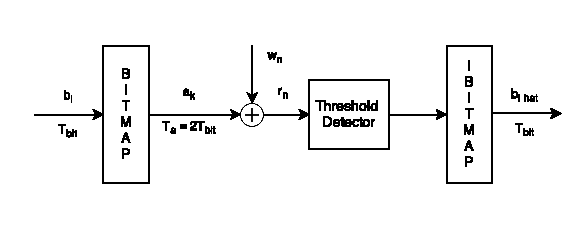
\includegraphics[width = 0.6\textwidth]{SC_uncoded}
	\caption{Block diagram for the simulation of a Single Carrier uncoded QPSK}
	\label{fig:problem1_scuncoded}
\end{figure}

\begin{figure}
	\centering
	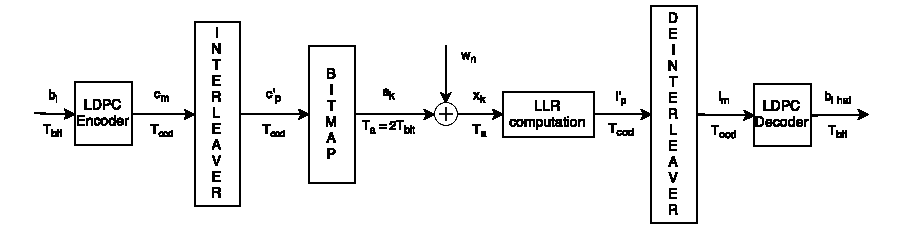
\includegraphics[width = \textwidth]{SC_coded}
	\caption{Block diagram for the simulation of a Single Carrier coded QPSK}
	\label{fig:problem1_sccoded}
\end{figure}

The uncoded Single Carrier QPSK configuration was implemented as described in Figure~\ref{fig:problem1_scuncoded}. First of all, a random data stream is created using the \texttt{randi} function. For the BER simulations, $L_{bits} = 2^{24}$ bits were used for every SNR. While this number of bits is unnecessarily large to estimate the Bit Error Rate for the lower SNRs, it was decided not to optimize it because the simulations were sufficiently fast. This is due to the lightweight operations the script has to perform: after the initial bitmapping of the bits to obtain the QPSK symbols, the channel only adds noise and there is no need to perform any convolution with an impulse response since the channel is ideal. Finally, the receiver only computes a thresholding and an inverse bit mapping. The results of the simulation can be seen in Figure~\ref{fig:problem1_pbit}, and coincide with those obtained in the previous homework. % TODO insert this reference to the old homework???

% TODO Insert stuff about the bitmap? We did it as required, should we really explain this?

When using coding, the script has to perform more complex computations that are illustrated in Figure~\ref{fig:problem1_sccoded}. The random bit sequence needs to have a length compatible with both the encoder and the interleaver. In fact, the provided LDPC encoder requires information words to have length $L_{iw} = 32400$ bits, and encodes them into codewords of length $L_{cw} = 64800$ bits. This doesn't represent a limitation, as shorter information words may be padded to reach the desired length, encoded and de-padded at the receiver, once decoded. In order to simplify things, however, it was decided to only send information words that have length that is a multiple of the information word length required by the encoder. Additionally, the interleaver matrix was given dimensions of $30 \times 36$ in order to facilitate the process of interleaving the codeword bits. Since $30 \cdot 36 = 1080$ is a divisor of the length of the codewords, when codewords of length $L_{cw} = k \cdot 64800, k \in \mathbb{N^{+}}$ need to be interleaved, the interleaver uses a number of matrices equal to $\frac{L_{cw}}{30\cdot36} = 60 \cdot k$, thus ensuring that all matrices will be filled completely and that no additional padding is required. Using this setup, if the desired length is $L_d$, the nearest compatible length of the message to be sent can be computed using the expression $L_{msg} = \lceil \frac{L_{d}}{32400} \rceil \cdot 32400$. Once the bits are generated, encoded and interleaved, they are translated into symbols using the QPSK bitmap and sent through the channel, that adds the noise $w_k \sim \mathcal{CN}(0, \sigma_w^2)$. If $\sigma^2_I = \frac{\sigma^2_w}{2}$ is the variance of the real and imaginary components of the noise and $\rho_k = \rho_{k,I} + j \rho_{k,Q}$ is the symbol received at time k, at the receiver side the Log Likelihood Ratio (LLR) can be computed using the following expression:
\begin{equation}
	l'_p =
	\begin{dcases}
	\frac{2 \rho_{k,I}}{\sigma_I^2}, \quad p = 2k \\
	\frac{2 \rho_{k,Q}}{\sigma_I^2}, \quad p = 2k +1
	\end{dcases}
\end{equation}
% TODO: more about what the LLR is and on how it works?
If the symbol period is $T_a$, the LLR vector will have bit period equal to $T_{cod} = \frac{T_a}{2}$, as one value of the LLR corresponds to one bit of the encoded message at the transmitter side. In order to get back to the actual correspondence with the original message $b_l$, it is necessary to deinterleave the LLR and to decode it. By feeding the LLR to the decoder, we are using it in its \emph{soft decoding} mode: the decoder will make use of the likelihood associated to the value of each bit, instead of the ``hard value'' of the bits, to perform the decoding. % TODO Necessary?
The output of the decoder, $\hat{b}_l$, is the final decision on the received symbols. This is the vector that is compared to $b_l$ in order to compute the probability of bit error. The results can once again be seen in Figure~\ref{fig:problem1_pbit}. 

% BER plot for coded vs uncoded QPSK
\begin{figure}
	\centering
	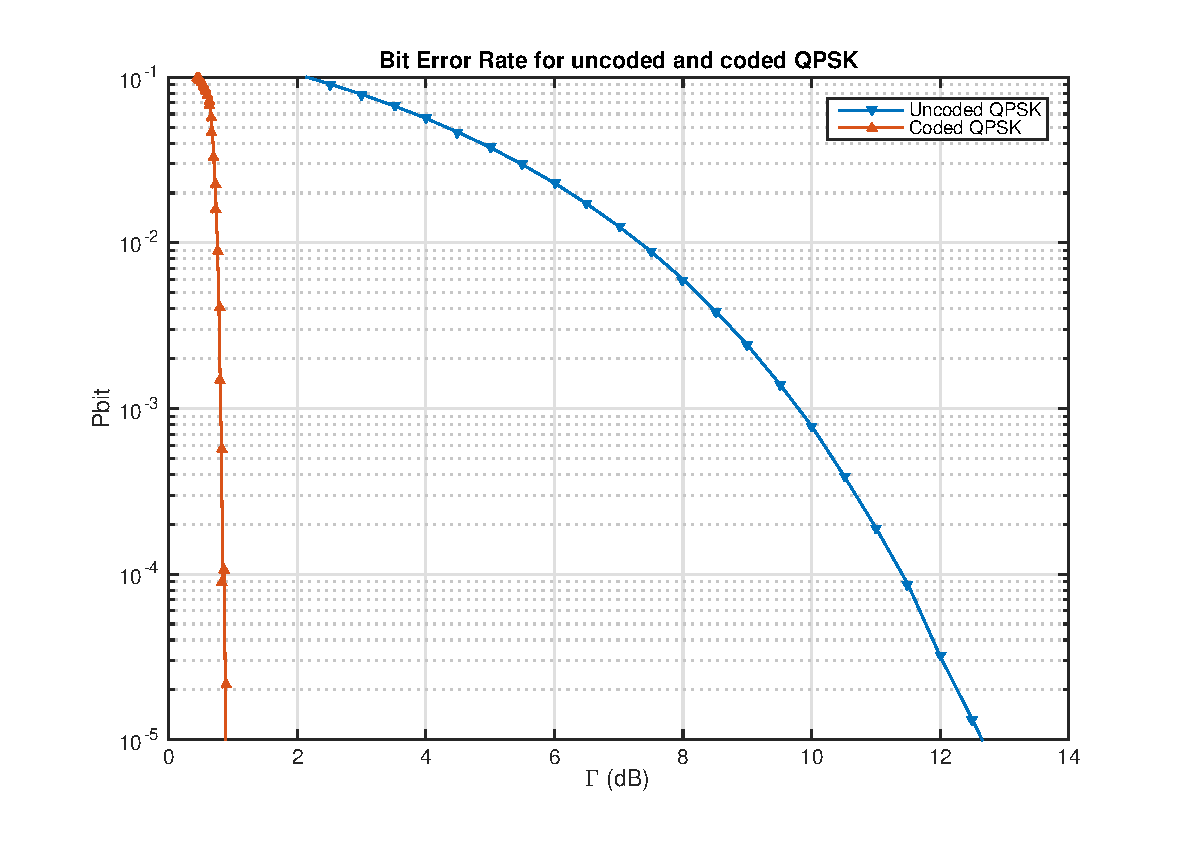
\includegraphics[width = 0.6\textwidth]{problem1}
	\caption{BER simulation results for coded vs. uncoded QPSK}
	\label{fig:problem1_pbit}
\end{figure}



%%%%%%%%%%%%%%%%%%%%%%%%%%%%%%%%%%%%%%%%%
%%%%%%%%%%%%%% PROBLEM 2 %%%%%%%%%%%%%%%%
%%%%%%%%%%%%%%%%%%%%%%%%%%%%%%%%%%%%%%%%%

\section*{Problem 2}
The setup used for the simulations with the DFE only varies when considering the coded and uncoded setting: using the actual or estimated impulse response only reflects changes on the DFE setting (i.e., the impulse response and the noise variance). 

The simulations that do not use channel coding follow the block scheme in %Figure~\ref

The timing phase $t_0 = 5$ was determined as the index of the first non-zero sample of the channel impulse response ${h_i}$.

% Required stuff:
% Setting of the DFE (as of the previous homework)
% In the HW text it is said that this should be re-designed for every SNR, specify this is what we do (the values of sigma_w are needed by the DFE and vary for each of the SNRs)
% Write values of t0, M1, M2 and D used. Say that these will be used for every SNR
% Write expressions of LLRs for the known channel, specifying that the noise that is being taken into account is the actual channel noise. There also is no ISI noise as it is assumed to have been cancelled by the DFE, specify this!
% Write expression of LLRs for the estimated channel. Specify that we use the estimated channel noise, as it is the only thing the receiver actually knows. 



\begin{figure}
	\centering
	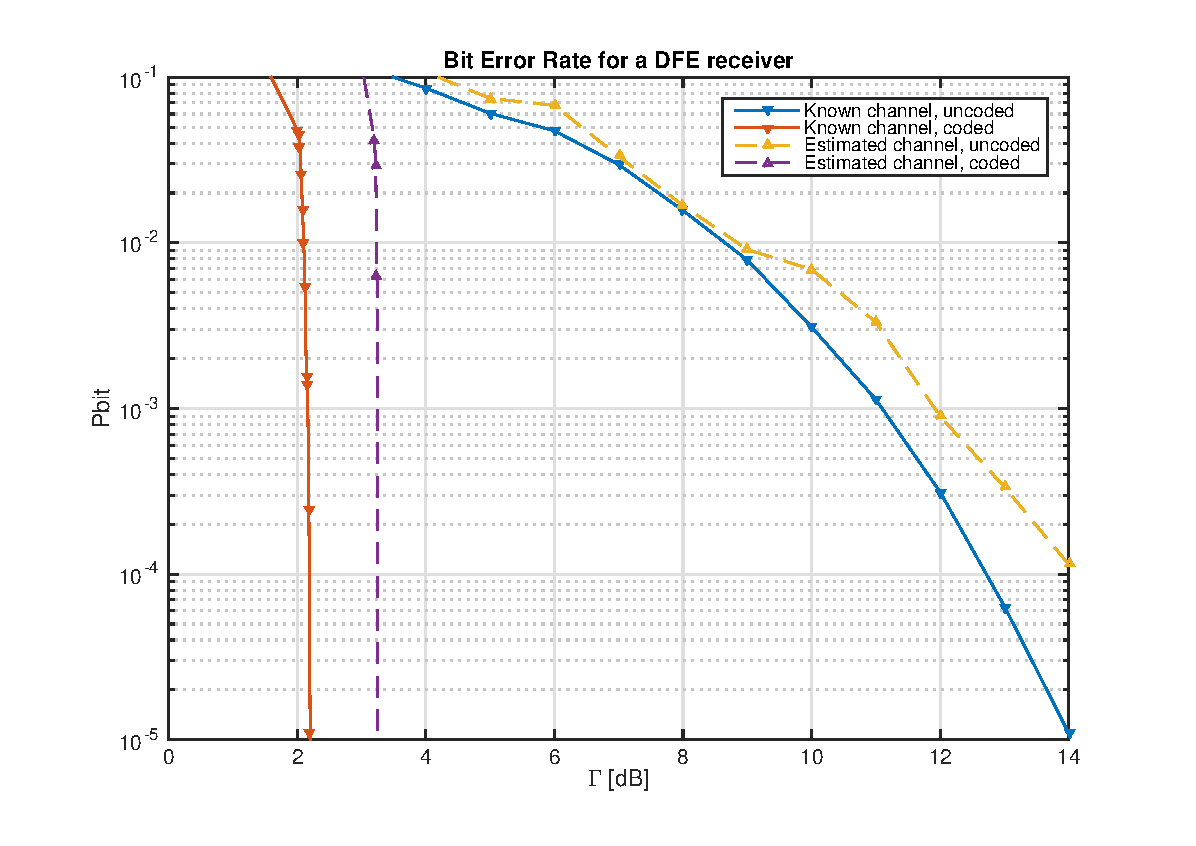
\includegraphics[width = 0.6\textwidth]{problem2}
	\caption{BER simulation for a DFE receiver using the estimated and actual channel ir, with or without coding}
	\label{fig:problem2_pbit}
\end{figure}

%%%%%%%%%%%%%%%%%%%%%%%%%%%%%%%%%%%%%%%%%
%%%%%%%%%%%%%% PROBLEM 3 %%%%%%%%%%%%%%%%
%%%%%%%%%%%%%%%%%%%%%%%%%%%%%%%%%%%%%%%%%
\section*{Problem 3}

\begin{figure}
	\centering
	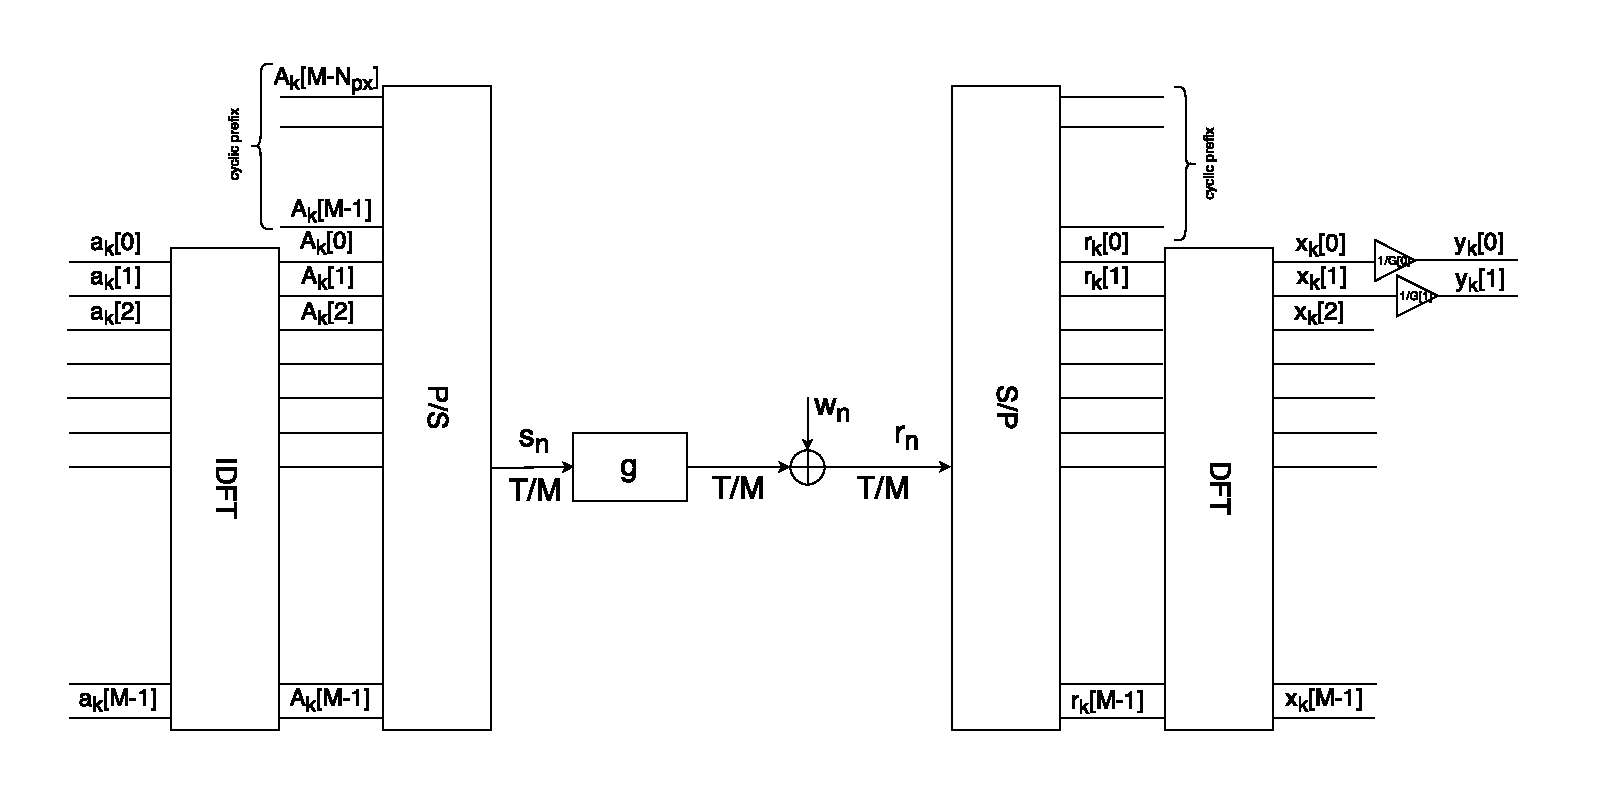
\includegraphics[width = 0.8\textwidth]{OFDM}
	\caption{OFDM system structure}
	\label{fig:OFDM}
\end{figure}

\subsection*{Transmitter structure}
Figure~\ref{fig:OFDM} shows the structure of an OFDM transmitter - receiver and a model for the channel. The $a$ symbols could represent either coded or uncoded bits, as in previous problems. Let $k$ be the block index. The symbols are taken in chunks of $\ofdM = 512$ in order to compose the vector $a_k[i], i \in [0, \ofdM - 1]$. The IDFT is then computed to get $A_k[i], i\in [0, \ofdM-1]$. At this step a cyclic prefix (whose role will be explained after having introduced the receiver) is introduced, i.e. for each block the last $N_{px} = 7$ symbols are repeated at the beginning of the $A_k$ vector. Finally the symbols $A_k[i]$ are serialized in order to obtain the vector $s_n$, which is sent through the channel.

% This consideration on SNR
As usual the SNR is defined as $\Gamma = \frac{\sigma_s^2 E_h}{\sigma_w^2}$. With an OFDM system, however, the meaning of $\sigma_s^2$ changes. As mentioned, the transmitter performs an IDFT, which is
\begin{equation}
	A_k[\ell] = \frac{1}{\ofdM} \sum_{i = 0}^{\ofdM - 1} W_{\ofdM}^{-i\ell} a_k[i], \quad \ell = 0, 1, \dots, \ofdM-1,
\end{equation}
Therefore we have 
% see formula 9.35, 9.38, 9.39
\begin{equation}
	\sigma_s^2 = \dfrac{\sigma_a^2}{\ofdM}.
\end{equation}

The MATLAB function \texttt{ifft} performs the IDFT with the correct scaling factor of $1/\ofdM$. Therefore, to compute the power of the noise introduced by the channel we must consider the SNR as
\begin{equation}
	\Gamma = \dfrac{\sigma_a^2 E_h}{\ofdM \sigma_w^2},
\end{equation}
that yields
\begin{equation}
	\sigma_w^2 = \dfrac{\sigma_a^2 E_h}{\ofdM \Gamma}.
\end{equation}

\subsection*{Receiver structure}
The receiver of OFDM has the structure of Figure~\ref{fig:OFDM}. The timing phase is $t_0 = 5 T$, which corresponds to the beginning at the receiver of the cyclic prefix. For each block of $\ofdM + N_{px}$ symbols the first $N_{px}$ are discarded and the DFT is then computed only on the $\ofdM$ samples which don't belong to the cyclic prefix of each block. Let the vector of symbols before the DFT be $\mathbf{r}_k$, with $k$ the block index, and $\mathbf{g}_{c,\ofdM}$ be the channel impulse response, of length $N \le N_{px} - 1$, padded with zeros in order to have a vector of length $M$. Then it is possible to define the circulant matrix of the IDFT of the transmitted symbols $a_k[i], i = 0, \dots, \ofdM$ as
\begin{equation}
	\boldsymbol{\Xi} = 
	\begin{bmatrix}
		A_k[0] & A_k[\ofdM - 1] & \dots & A_k[1] \\
		A_k[1] & A_k[0] & \dots & A_k[2] \\
		\vdots & \vdots & \ddots & \vdots \\
		A_k[\ofdM - 1] & A_k[\ofdM - 2] & \dots & A_k[0] \\
	\end{bmatrix}
\end{equation}
and express $\mathbf{r}_k$ as
\begin{equation}
	\mathbf{r}_k = \boldsymbol{\Xi} \mathbf{g}_{c,\ofdM} + \mathbf{w}_k
\end{equation}
with $w_k$ a vector of AWGN samples. Then the receiver performs the DFT using an $\ofdM \times \ofdM$ DFT matrix $\DFTmat$ in order to get $ \mathbf{x}_k = \DFTmat \mathbf{r}_k$. In particular, let's consider the following 
\begin{eqnarray}
	 \mathbf{x}_k & = & \DFTmat \mathbf{r}_k = \DFTmat \boldsymbol{\Xi} \DFTmat^{-1} \DFTmat \mathbf{g}_{c,\ofdM} + \DFTmat \mathbf{w}_k\\
	  & = & \mathrm{diag}\{\mathbf{a}_k\} \mathbf{G}_c + \mathbf{W}_k
\end{eqnarray}
because $\boldsymbol{\Xi}$ is a circulant matrix. $\mathbf{W}_k$ is a still a vector of independent Gaussian random variables, each of them with variance $\sigma_W^2 = \ofdM \sigma_w^2$. 

This procedure removes the effects of ICI and ISI introduced by the non-ideal channel, and it is followed by a scaling of the received symbols on each channel in order to get the same constellation of the transmitter. In particular for each subchannel $i$ 
\begin{equation}
	y_k[i] = \frac{x_k[i]}{G_c[i]} = a_k[i] + \frac{W_k[i]}{G_c[i]}
	\label{eq:yofdm}
\end{equation}
Finally the receiver performs a decision. If the transmitted bits are uncoded, it uses a threshold detector on each subchannel and an inverse bitmap. Note that the performances of an uncoded OFDM system are negatively affected by the presence of subchannels in which the frequency response $G_c$ of the channel exhibits a great attenuation, because in that subchannels the received symbols are zeros or below noise level. 
% TODO fix this sentence

If the coded option is used, instead, the data which would be lost because of frequency response attenuation in that subchannel can be recovered with coding. In particular given the observed symbol $y_k[i]$ defined in~\eqref{eq:yofdm} let the variance of the noise per component of subchannel $i$ be $\sigma_I^2 = 0.5 \sigma_W^2/|G_c[i]|^2 = 0.5 \ofdM \sigma_w^2/|G_c[i]|^2$. Then the log-likelihood ratios (LLR) of each subchannel are defined as
\begin{eqnarray}
	\mathrm{LLR}_I = \frac{2\Re(y_k[i])}{\sigma_I^2} = 2\Re(y_k[i]) \frac{|G_c[i]|^2 }{0.5 \ofdM \sigma_w^2} \\
	\mathrm{LLR}_Q = \frac{2\Im(y_k[i])}{\sigma_I^2} = 2\Im(y_k[i]) \frac{|G_c[i]|^2 }{0.5 \ofdM \sigma_w^2} \\
\end{eqnarray}

\subsection*{Channel estimation for OFDM}
In order to perform the operations described in the previous section, the receiver has to know the frequency response of the channel and the noise power of each subchannel. In this homework the simulation of the BER has been carried out both with an a-priori perfectly known channel and with an estimated channel. 
%% TODO give reasons behind this kind of spacing
The estimation of the channel has to be performed with $L_{ts} = 32$ pilot symbols, all in block $0$. For a given SNR $\Gamma$ computed with the data power $\sigma_a^2 = 2$, then the pilot symbols have $\sigma_{ts} = 4$ as required. The pilot symbols $a_{ts}[i]$ are inserted in the subchannels $i \in \mathcal{T}_{ind} = \{ 0, 15, 31, \dots, 497 \}$, i.e. with a spacing of $\ofdM/L_{ts}$ subchannels between each other. The other $\ofdM - L_{ts}$ symbols can be data or anything else, they are not used for the estimation. At the receiver, after the DFT, the $L_{ts}$ $x_0[i], i \in \mathcal{T}_{ind}$, are divided by the corresponding pilot symbol $a_{ts}[i]$ in order to get $\tilde{G}[i] = G_c[i] + W_0[i]/a_{ts}[i]$. Let $\boldsymbol{\Omega}$ be a realization of the vector $\tilde{\mathbf{G}}_i = \tilde{G}[i], i\ \in \mathcal{T}_{ind}$. 
Then the procedure exploits the fact that the channel impulse response can have at most $N \le N_{px} + 1 = 8$ taps, so the uncorrelated samples of the frequency response $G_c[i]$ are at most 8. In particular if $\mathbf{G}_c$ is seen as the DFT of the channel impulse response then
\begin{equation}
	\mathbf{G}_c = \DFTmat_{\ofdM \times \ofdM} \mathbf{g}_{c,\ofdM} = \DFTmat_{\ofdM \times N_{px} + 1} \, \mathbf{g}_c
\end{equation}
By choosing the 32 subchannels with pilot symbols (i.e. for $ i\ \in \mathcal{T}_{ind}$) it is possible to define a matrix $\boldsymbol{\tilde{\mathcal{F}}}$ of size $L_{ts} \times N_{px} + 1$ with the first $N_{px} + 1$ columns of $\DFTmat_{\ofdM \times \ofdM}$ (at most the ones which are not multiplied by zero), at rows $ i\ \in \mathcal{T}_{ind} $. Let $\tilde{\mathbf{W}}_i = W_0[i]/a_{ts}[i], i\ \in \mathcal{T}_{ind}$ be the vector of noise samples which correspond to the subchannels with pilot symbols. Then it is possible to write $\mathbf{\tilde{G}}$ as
\begin{equation}
	\mathbf{\tilde{G}} = \boldsymbol{\tilde{\mathcal{F}}}\mathbf{g}_{c} + \tilde{\mathbf{W}}
\end{equation}
Given an observation $\boldsymbol{\Omega}$, the vector $\mathbf{g}_{c}$ can be finally found by applying the LS method to minimize the difference
\begin{equation}
	\boldsymbol{\tilde{\mathcal{F}}}\mathbf{g}_{c} - \boldsymbol{\Omega}
\end{equation}
which is
\begin{eqnarray}
	\boldsymbol{\Phi} = \boldsymbol{\tilde{\mathcal{F}}}^H \boldsymbol{\tilde{\mathcal{F}}} \\
	\boldsymbol{\theta} = \boldsymbol{\tilde{\mathcal{F}}}^H \boldsymbol{\Omega} \\ 
	\hat{\mathbf{g}}_{c} = \boldsymbol{\Phi}^{-1} \boldsymbol{\theta} 
\end{eqnarray}
Finally let $\hat{\mathbf{g}}_{c, \ofdM}$ be $\hat{\mathbf{g}}_{c}$ with a zero padding in order to make it of 512 samples. In order to estimate the frequency response at each subchannel the DFT is applied on $\hat{\mathbf{g}}_{c, \ofdM}$, so $\hat{\mathbf{G}} = \mathcal{F}[\hat{\mathbf{g}}_{c, \ofdM}]$. 

The noise power is estimated as 
\begin{equation}
	\hat{\sigma_w^2} = \frac{1}{L_{ts}} \sum_{i \in \mathcal{T}_{ind}} |a_{ts}[i]\hat{G[i]} - x_0[i]|^2
\end{equation}
provided that $a_{ts}[i]\hat{G[i]} - x_0[i]$ has zero mean.

\begin{thebibliography}{10}

\bibitem{bc}
Benvenuto, Cherubini, Algorithms for Communications Systems and their Applications, Wiley, 2004

\end{thebibliography}

\end{document}
